\documentclass{ieeeaccess}
\usepackage{cite}
\usepackage{amsmath,amssymb,amsfonts}
\usepackage{graphicx}
\usepackage{booktabs}
\usepackage{url}
\urlstyle{same}
\usepackage{algorithmic}
\usepackage{amsthm}
\usepackage{etoolbox}
% Avoid stretching the gap before a single author biography on the final page.
\patchcmd{\IEEEbiographynophoto}{\vskip 4\baselineskip plus 1fil minus 0\baselineskip}{\vskip 2\baselineskip}{}{}
\newtheorem{proposition}{Proposition}
\newcommand{\ind}{\mathbf{1}}
\newcommand{\Rscore}{\mathcal{R}}
\begin{document}
\history{Manuscript prepared for peer review, September 2026.}
\doi{To be assigned upon publication}
\vol{unassigned}\year{2026}
\title{PROXIMA: Auditing Proxy Decisions and Within-Segment Disagreement in Online Experiments}
\author{\uppercase{Avinash Amudala}\authorrefmark{1}}
\address[1]{Independent Researcher (e-mail: aa9429@g.rit.edu)}
\tfootnote{Author ORCID: 0009-0000-7226-6156. An earlier version of this work is available as arXiv:2604.14352.}
\markboth{Amudala: PROXIMA}{Amudala: PROXIMA}
\corresp{Corresponding author: Avinash Amudala (e-mail: aa9429@g.rit.edu).}
\begin{abstract}
Proxy metrics can agree with an outcome at the population level while supporting incorrect decisions for particular user segments. This paper presents PROXIMA, a descriptive auditing framework that reports effect correlation, decision agreement, and within-segment directional disagreement separately and combines them in a transparent weighted score. The framework distinguishes local proxy error from disagreement with an overall launch decision, specifies metric orientation and zero-effect behavior, and separates decision accuracy from shipment precision. Evaluation uses four fully specified synthetic settings with independent training and test experiment corpora and an observed-data illustration using the Criteo uplift dataset. Across 100 independent repetitions, the default composite achieves mean held-out decision agreement of 0.920 in the balanced simulation, compared with 0.802 for correlation-based selection and 0.941 for decision-agreement selection. Its local error is lower than those two comparators in that setting, illustrating a trade-off between overall and subgroup decisions. Under an imposed calibration shift, composite agreement falls to 0.544, demonstrating that historical scores do not guarantee transportability. In Criteo, all 50 random partitions favor treatment, so perfect proxy agreement is also achieved by always shipping and does not establish generalization across interventions. The contribution is an auditable diagnostic and reproducible characterization of its limitations, rather than an optimal surrogate estimator or a calibrated probability of future reliability.
\end{abstract}
\begin{keywords}
A/B testing, decision evaluation, online controlled experiments, proxy metrics, reproducibility, subgroup analysis.
\end{keywords}
\titlepgskip=-21pt
\maketitle

\section{Introduction}
\PARstart{O}{nline} controlled experiments estimate the effects of product changes, but a decision-relevant outcome can be slow or expensive to observe. Practitioners therefore use an earlier or more sensitive proxy. The methodological challenges of this practice extend beyond testing whether a treatment effect differs from zero: the proxy must also answer the intended decision question \cite{kohavi,larsen}.\footnote{AI-assisted drafting \cite{codex}; see Acknowledgment.}

Three questions motivate this work. Do proxy effects track outcome effects across past experiments? Do they support the same overall launch decisions? Does their agreement persist within relevant user segments? These questions are related but are not equivalent. Correlation is invariant to a constant offset, which can change the signs of effects. Overall agreement can coexist with local disagreement. Moreover, a segment can legitimately respond differently from the population while its proxy remains locally accurate.

PROXIMA reports all three dimensions and provides an optional weighted summary for comparing existing proxies. The summary is intentionally simple: its purpose is to make a decision criterion inspectable, not to replace statistical surrogate construction. We evaluate both benefits and failure cases, including a setting in which the composite performs substantially worse after a distribution change. The study asks whether a local disagreement component changes the balance between overall and subgroup decision quality under controlled assumptions.

The contributions are: (1) an explicit distinction between within-segment proxy disagreement and disagreement with a population decision; (2) a reproducible audit implementation with specified handling of orientation, missing effects, and uncertainty; and (3) a held-out simulation comparison against component ablations and simple decision policies, accompanied by a carefully delimited observed-data illustration. A bounded weighted sum is not itself a new statistical estimator. The empirical contribution concerns how its components behave together and where their interpretation breaks down.

\section{Related Work and Scope}
Surrogate-index methods combine short-term measurements to estimate a longer-term treatment effect under assumptions about surrogacy and comparability \cite{athey}. Tripuraneni et al. construct proxy metrics using a historical experiment corpus and account for experiment noise in proxy selection \cite{tripuraneni}. Zhang et al. evaluate surrogate-based decisions using a corpus of Netflix experiments \cite{zhang}. These approaches motivate evaluating decisions on experiments distinct from those used to select a metric.\footnote{AI-assisted drafting \cite{codex}; see Acknowledgment.}

PROXIMA addresses a narrower task: auditing a supplied set of proxy effect estimates. It does not estimate the causal relation between proxy and outcome, identify a sufficient surrogate, or learn an optimal proxy combination. Accordingly, the empirical comparisons here are between diagnostic selection rules using identical inputs. They are not performance comparisons against the surrogate-index or noise-aware optimization methods cited above.

The online experimentation literature also distinguishes statistical sensitivity from relevance to the outcome of interest \cite{larsen}. A precise proxy estimate can still support a poor decision if its effect is misaligned. Likewise, a noisy within-segment sign mismatch is not proof of a causal mechanism or of Simpson's paradox. We use the term \emph{local disagreement} for a descriptive mismatch and reserve causal or inferential interpretations for designs that justify them.

This manuscript revises the earlier PROXIMA preprint \cite{preprint}. The present evaluation replaces its headline numerical claims. In particular, the earlier KuaiRec workflow generated outcomes from assumed response distributions using user covariates; it did not provide observed long-term outcomes from randomized recommendation policies. KuaiRec is a valuable recommendation dataset \cite{kuairec}, but those generated outcomes are not used as independent real-world validation here. The current evidence consists of fully disclosed simulations and a separate Criteo analysis.

\section{Audit Definition}
\subsection{Inputs and Decision Rules}
Let $e=1,\ldots,E$ index experiments, $s$ index prespecified segments, and $p$ index candidate proxies. Denote estimated overall proxy and outcome effects by $\widehat\tau_{p,e}$ and $\widehat\tau_{y,e}$, with corresponding segment effects $\widehat\tau_{p,e,s}$ and $\widehat\tau_{y,e,s}$. With randomized assignment and suitable sampling assumptions, effects can be estimated by differences in treatment and control means. The audit itself accepts estimated effects and cannot establish the validity of their causal interpretation.\footnote{AI-assisted drafting \cite{codex}; see Acknowledgment.}

Specify the preferred direction $d_p\in\{-1,+1\}$ before inspecting evaluation outcomes. For example, a reduction in a delay metric is favorable. Write $x_{p,e}=d_p\widehat\tau_{p,e}$ and assume the outcome is oriented so a positive effect is favorable. Throughout the experiments, the decision rule is
\begin{equation}
 a_{p,e}=\ind\{x_{p,e}>0\},\qquad
 a_{y,e}=\ind\{\widehat\tau_{y,e}>0\}.
\end{equation}
An exact zero means no ship. This sign rule is an evaluation convention, not a recommendation to launch statistically inconclusive experiments. Production decisions may require uncertainty bounds, minimum practical effects, costs, and additional guardrails.

\subsection{Three Descriptive Components}
Define normalized Pearson correlation and decision agreement as
\begin{align}
 C_p&=\{1+\operatorname{corr}(x_{p,e},\widehat\tau_{y,e})\}/2,\\
 D_p&=E^{-1}\sum_e\ind\{a_{p,e}=a_{y,e}\}.
\end{align}
For eligible experiment--segment cells $\mathcal{I}$, define
\begin{equation}
 F_p=\frac{1}{|\mathcal{I}|}\sum_{(e,s)\in\mathcal{I}}
 \ind\{\ind[x_{p,e,s}>0]\ne\ind[\widehat\tau_{y,e,s}>0]\}.
\end{equation}
Thus $F_p$ compares the proxy with the outcome \emph{within the same segment}. It weights eligible cells equally rather than weighting by population size. Unequal segment sizes therefore change the interpretation: the score expresses an equal-cell audit objective, not total population harm.

The composite is
\begin{equation}
 \begin{aligned}
 \Rscore_p&=w_C C_p+w_D D_p+w_F(1-F_p),\\
 &w_C,w_D,w_F\geq0,\quad w_C+w_D+w_F=1.
 \end{aligned}
\end{equation}
The default weights are $(0.6,0.2,0.2)$, retained as a heuristic convention rather than estimated as optimal. All components and sample counts remain visible. A score of 0.8 is not an 80\% probability that the proxy is safe or that its next decision will be correct.

\begin{proposition}
When all components are defined, $\Rscore_p\in[0,1]$ and is nondecreasing in $C_p,D_p$ and nonincreasing in $F_p$. If every weight is strictly positive, $\Rscore_p=1$ if and only if $C_p=D_p=1$ and $F_p=0$; the analogous zero endpoint requires $C_p=D_p=0$ and $F_p=1$.
\end{proposition}
\begin{proof}
The score is a convex combination of three numbers in $[0,1]$. Its partial derivatives are $w_C,w_D,-w_F$. A positive-weight average reaches an endpoint only when every component reaches that endpoint. With a zero weight, the excluded component need not attain an endpoint.
\end{proof}
This elementary property establishes a consistent scale, not predictive validity. When correlation is undefined because effects are constant or too few, the implementation flags it and uses $C_p=0.5$ as an explicitly neutral convention. An absent local comparison makes the composite unavailable, rather than implicitly declaring zero fragility.

\subsection{Local Versus Population Disagreement}
A separate diagnostic replaces the local outcome in $F_p$ with the overall outcome. Call this quantity $G_p$. If an overall outcome is positive but a segment has proxy and outcome effects both negative, that cell contributes to $G_p$ but not $F_p$. Conversely, a positive proxy and negative local outcome can be missed by $G_p$ when the overall outcome is positive. Reporting the two quantities separately prevents local treatment heterogeneity from being mistaken for proxy error.

The observation of sign differences is descriptive. No individual segment is declared statistically unreliable in this study. Near-zero effects are particularly sensitive to sampling noise; an inferential extension would need a specified uncertainty rule and adjustment for the family of segment hypotheses being tested.

\subsection{Missingness and Uncertainty}
The participant-level implementation uses pairwise complete proxy--outcome observations and excludes experiment or segment comparisons with fewer than two observed units in either arm. Exclusions and effective counts are reported. This makes the calculation defined; it does not correct informative missingness. Constant-effect cases, empty cells, and absent classification denominators are handled explicitly.

A percentile bootstrap resamples experiments as blocks, carrying their segment effects with them. Every repeated draw retains its multiplicity. A participant-level implementation assigns each sampled copy a new experiment identifier before aggregation. This prevents repeated draws from being collapsed by the original identifier. Intervals condition on the measured effects and do not remove shared measurement error or guarantee transport across populations.

\subsection{Decision Evaluation}
We distinguish agreement $(TP+TN)/E$ from shipment precision $TP/(TP+FP)$. False-positive and false-negative rates are $FP/(FP+TN)$ and $FN/(TP+FN)$, respectively. A missing denominator is reported as undefined.

When the true outcome effect $\tau_{y,e}$ is known, decision regret is
\begin{equation}
 L=E^{-1}\sum_e |\tau_{y,e}|\,
 \ind\{a_{p,e}\ne\ind[\tau_{y,e}>0]\}.
\end{equation}
It is nonnegative and includes both harmful launches and missed benefits. In observed data, substituting an estimated outcome provides agreement with a measured reference, not with an omniscient oracle. The distinction matters when the reference effect is noisy.

\section{Experimental Design}
\subsection{Synthetic Experiment Corpora}
We generate effects directly under a Gaussian estimation model. No simulated row is described as an observed user or a real platform experiment. Each repetition contains 60 training experiments and 60 independent test experiments, with five equally weighted segments per experiment. We run 100 repetitions for each of four settings, using NumPy seed sequences derived from $(20260928,\text{setting index},\text{repetition})$.\footnote{AI-assisted drafting \cite{codex}; see Acknowledgment.}

For experiment $e$, draw a global outcome effect $g_e\sim N(0,0.12^2)$ and five deviations $u_{e,s}\sim N(0,h^2)$. Center the deviations within the experiment, $z_{e,s}=u_{e,s}-\bar u_e$, and set the true local outcome to $y_{e,s}=g_e+z_{e,s}$. This construction makes the equally weighted global effect exactly $g_e$.

There are four fixed candidate proxies. Their latent local effects are
\begin{align}
 q_{1,e,s}&=y_{e,s}+\eta_{e,s},\quad \eta_{e,s}\sim N(0,0.06^2),\\
 q_{2,e,s}&=y_{e,s}+0.12,\\
 q_{3,e,s}&=g_e-z_{e,s},\\
 q_{4,e,s}&\sim N(0,0.20^2).
\end{align}
These candidates represent an approximately faithful proxy, a calibration offset, reversed subgroup deviations, and an unrelated signal. The third retains the overall latent effect while changing local effects. Candidate order is fixed as written; exact ties select the first candidate.

Observed effects add estimation noise:
\begin{align}
 \widehat y_{e,s}&=y_{e,s}+\epsilon_{e,s},\\
 \widehat q_{p,e,s}&=q_{p,e,s}+0.3\epsilon_{e,s}
                  +\sqrt{0.91}\,\xi_{p,e,s},
\end{align}
where $\epsilon$ and $\xi$ are mutually independent $N(0,\sigma^2)$ variables before the shared component is added. Thus marginal proxy and outcome noise variances are equal and their correlation is 0.3. Global estimates average the five local estimates. Test decisions use the observed proxy, while evaluation uses the true outcome. The measured test outcome is never used to select the proxy or evaluate its true decision loss.

The balanced setting uses $(\sigma,h)=(0.04,0.08)$; the heterogeneous setting uses $(0.04,0.20)$; the noisy setting uses $(0.12,0.08)$. The shifted setting has balanced training conditions but adds 0.20 to the first candidate's latent effects at test time. This is a deliberately targeted failure case, not a fitted model of deployment drift. The settings were specified for this revision and are not a preregistered or exhaustive benchmark.

\subsection{Selection Rules and Reporting}
Each rule chooses one proxy using only training effects. Comparators use correlation alone, decision agreement alone, local agreement alone, equal weights, and a composite without the local component $(0.75,0.25,0)$. We also evaluate every fixed candidate, uniform selection among the four candidates, always ship, and never ship. Uniform selection is the exact average of the four candidates' test metrics, not an assumed 50\% success rate.

We report global decision agreement, regret, and local decision error against known truth on test experiments. The local metric asks whether each segment's own proxy decision matches its own outcome decision; it is not an estimate of harm caused by an overall launch. Uncertainty bars are 95\% $t$ intervals over independent repetition means. Paired differences use the same training and test corpus for both rules. These exploratory Monte Carlo intervals are not simultaneous confidence statements over all comparisons and do not address uncertainty about the chosen data-generating model.

\subsection{Observed-Data Illustration}
The Criteo uplift dataset contains randomized advertising treatment assignments and observed visit and conversion labels \cite{criteo,diemert}. It pools data without exposing a corpus of identified interventions for our analysis. We therefore use it as one pooled treatment comparison, not as 50 independently designed interventions.

The downloaded file contains 13,979,592 rows. The first 100,000 rows determine three quartile boundaries of anonymized feature $f_0$ and are excluded from the analysis. The remaining 13,879,592 rows are assigned to 50 random partitions with seed 42, preserving original treatment assignments. The fixed boundaries are 20.599416, 22.959279, and 24.667063. Four resulting feature segments are used within each partition. Visit is the only candidate proxy; conversion is the observed outcome. Exposure is not relabeled as watch time, and conversion is not described as measured retention.

The 1,000-resample bootstrap in this illustration describes variation from resampling the constructed partitions. The partitions share a pooled treatment setting and are not evidence about variation across different product interventions. Since both labels are observed without the temporal experiment corpus needed for long-term validation, this illustration does not establish that visit predicts future retention or lifetime value.

\section{Results}
\begin{table*}[t]
\caption{Mean held-out decision agreement across 100 repetitions. All entries are generated from recorded simulation outputs.}
\label{tab:agreement}\centering% Generated by scripts/build_journal_assets.py; do not edit.
\begin{tabular}{lrrrr}
\toprule
Method & Balanced & Heterog. & Noisy & Shifted \\
\midrule
PROXIMA & 0.920 & 0.920 & 0.855 & 0.544 \\
Correlation & 0.802 & 0.784 & 0.804 & 0.804 \\
Decision only & 0.941 & 0.948 & 0.862 & 0.841 \\
Local only & 0.919 & 0.920 & 0.833 & 0.540 \\
Equal weights & 0.919 & 0.920 & 0.854 & 0.540 \\
No local component & 0.947 & 0.952 & 0.866 & 0.919 \\
Uniform proxy & 0.758 & 0.756 & 0.727 & 0.659 \\
Always ship & 0.503 & 0.496 & 0.501 & 0.486 \\
Never ship & 0.497 & 0.504 & 0.500 & 0.514 \\
\bottomrule
\end{tabular}

\end{table*}
\begin{table*}[t]
\caption{Mean held-out local decision error. Lower values indicate fewer within-segment disagreements with known simulated truth.}
\label{tab:local}\centering% Generated by scripts/build_journal_assets.py; do not edit.
\begin{tabular}{lrrrr}
\toprule
Method & Balanced & Heterog. & Noisy & Shifted \\
\midrule
PROXIMA & 0.153 & 0.100 & 0.290 & 0.403 \\
Correlation & 0.315 & 0.387 & 0.335 & 0.321 \\
Decision only & 0.281 & 0.490 & 0.323 & 0.365 \\
Local only & 0.149 & 0.100 & 0.252 & 0.404 \\
Equal weights & 0.149 & 0.100 & 0.269 & 0.404 \\
No local component & 0.321 & 0.591 & 0.342 & 0.353 \\
Uniform proxy & 0.321 & 0.357 & 0.355 & 0.387 \\
Always ship & 0.498 & 0.500 & 0.502 & 0.507 \\
Never ship & 0.502 & 0.500 & 0.498 & 0.493 \\
\bottomrule
\end{tabular}

\end{table*}
\begin{figure*}[t]
\centering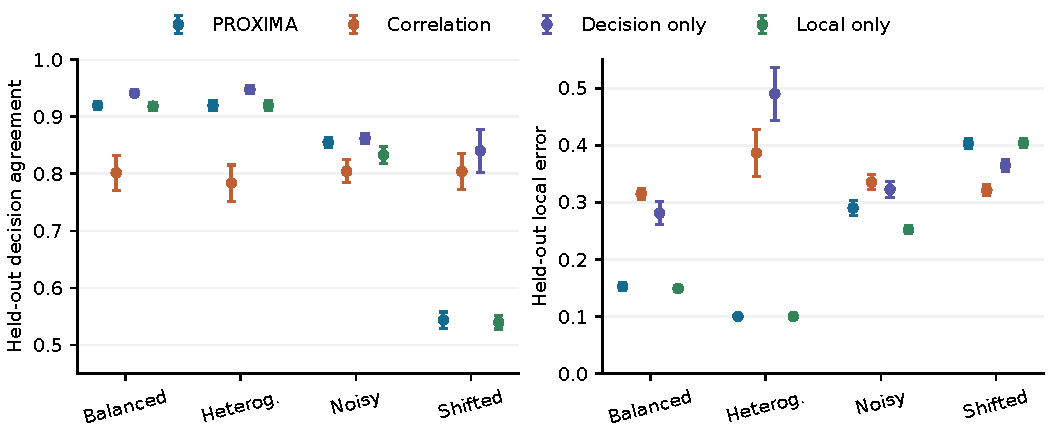
\includegraphics[width=.96\textwidth]{generated/simulation.pdf}
\caption{Global and local test outcomes. Bars show 95\% Monte Carlo intervals over repetition means. The calibration-shift setting is an explicit failure case.}
\label{fig:simulation}
\end{figure*}

\subsection{A Trade-off Between Overall and Local Decisions}
Tables~\ref{tab:agreement} and \ref{tab:local} show that adding the local component changes the selected proxy and the decision objective. In the balanced setting, PROXIMA achieves global agreement of 0.920, compared with 0.802 for correlation-only selection and 0.941 for decision-only selection. Its local error is 0.153, compared with 0.315 and 0.281, respectively. Thus the composite improves both outcomes over correlation in this constructed setting but exchanges some global accuracy for better local accuracy relative to decision-only selection.\footnote{AI-assisted drafting \cite{codex}; see Acknowledgment.}

The local-only comparator is competitive with the composite. The results do not establish that the default weighting is optimal or that every component is necessary for every objective. A user concerned only with overall sign decisions could reasonably prefer a different rule. Figure~\ref{fig:simulation} shows that these trade-offs persist with greater heterogeneity and change as observation noise increases.

\subsection{Failure Under Calibration Shift}
In the shifted setting, the default composite's global agreement falls to 0.544 while correlation-only selection reaches 0.804 and decision-only selection reaches 0.841. The shift targets the candidate that local-aware rules frequently prefer in training. This makes the case diagnostic of non-transportability, rather than a general ranking of robustness methods. It demonstrates that historical agreement cannot substitute for assumptions about future proxy behavior.

\begin{table*}[t]
\caption{Paired differences: PROXIMA minus correlation-only selection, with exploratory 95\% Monte Carlo intervals. A positive agreement difference and a negative local-error difference favor PROXIMA.}
\label{tab:paired}\centering\begin{tabular}{lrr}
\toprule
Scenario & Agreement difference & Local-error difference \\
\midrule
Balanced & +0.118 [+0.087, +0.148] & -0.162 [-0.173, -0.151] \\
Heterogeneous & +0.136 [+0.103, +0.169] & -0.286 [-0.328, -0.245] \\
Noisy & +0.051 [+0.032, +0.070] & -0.045 [-0.060, -0.030] \\
Shifted & -0.260 [-0.294, -0.226] & +0.082 [+0.072, +0.092] \\
\bottomrule
\end{tabular}

\end{table*}
\begin{table*}[t]
\caption{Mean regret in simulated outcome-effect units. Lower is better. Regret includes missed benefits as well as harmful launches.}
\label{tab:regret}\centering% Generated by scripts/build_journal_assets.py; do not edit.
\begin{tabular}{lrrrr}
\toprule
Method & Balanced & Heterog. & Noisy & Shifted \\
\midrule
PROXIMA & 0.001 & 0.002 & 0.005 & 0.036 \\
Correlation & 0.010 & 0.012 & 0.009 & 0.010 \\
Decision only & 0.001 & 0.001 & 0.005 & 0.010 \\
Local only & 0.002 & 0.002 & 0.007 & 0.036 \\
Equal weights & 0.002 & 0.002 & 0.005 & 0.036 \\
No local component & 0.001 & 0.001 & 0.004 & 0.004 \\
Uniform proxy & 0.018 & 0.018 & 0.019 & 0.026 \\
Always ship & 0.048 & 0.048 & 0.048 & 0.049 \\
Never ship & 0.049 & 0.047 & 0.047 & 0.047 \\
\bottomrule
\end{tabular}

\end{table*}
Table~\ref{tab:paired} reports paired contrasts instead of interpreting overlap between separate intervals. Table~\ref{tab:regret} confirms that the methods' ordering depends on the target loss, not just on the numerical spread of their scores. All fixed-candidate results, selection frequencies, component scores, and comparator contrasts are included in the reproducibility files.

\subsection{What the Criteo Illustration Can Establish}
\begin{table}[t]
\caption{Criteo visit--conversion illustration. The interval is conditional on the random partitions and is not an interval over independent interventions.}
\label{tab:criteo}\centering\begin{tabular}{lr}
\toprule
Quantity & Value \\
\midrule
Analysis rows & 13,879,592 \\
Random partitions & 50 \\
Pearson correlation & 0.055 \\
Decision agreement & 1.000 \\
Local disagreement & 0.230 \\
Composite score & 0.670 \\
Conditional 95\% interval & [0.572, 0.757] \\
Always-ship agreement & 1.000 \\
Negative partitions & 0 \\
\bottomrule
\end{tabular}

\end{table}
The revised analysis gives a composite score of 0.670 and local disagreement of 0.230 (Table~\ref{tab:criteo}). Every partition has a positive measured conversion effect. Visit-based decisions therefore agree with the reference in all 50 partitions, but an always-ship policy does so as well. There are no negative partitions from which to estimate a false-positive rate. This example shows why perfect aggregate agreement in an imbalanced evaluation set is weak evidence of discriminative ability.

The near-zero correlation across partitions concerns variation among estimates of the pooled treatment comparison. It should not be interpreted as evidence that the same proxy has near-zero correlation with outcomes across a genuinely heterogeneous corpus of interventions. Similarly, local sign disagreements can reflect noisy estimates rather than reproducible subgroup-specific failures.

\section{Practical Use and Limitations}
An audit should begin with an explicit decision objective, an outcome horizon, a preferred direction for each metric, and prespecified segments. Report the component scores and effective sample counts before using the composite. Select weights without looking at the evaluation corpus and measure performance on held-out experiments. Include constant decision policies so that class imbalance does not create a misleading impression of predictive success.\footnote{AI-assisted drafting \cite{codex}; see Acknowledgment.}

Several limitations constrain the present evidence. First, the default weights are heuristic and the simulation candidates were chosen to expose particular distinctions. The study cannot establish an optimal general-purpose metric selection policy. Second, estimated treatment-effect correlations contain measurement error; PROXIMA does not denoise them. Shared sampling error can create apparent agreement. Third, sign decisions discard effect magnitude and statistical uncertainty. Regret and uncertainty-aware policies should therefore accompany any practical deployment assessment.

Fourth, equal weighting of segment cells may overemphasize small groups or underrepresent population-level cost. Fifth, the descriptive fragility statistic is not a multiple-testing procedure. Data-dependent discovery of segments would require additional safeguards and independent evaluation. Sixth, the real-data illustration lacks identifiers for distinct interventions and observed long-horizon outcomes. It cannot establish cross-domain generalization or replace a production experiment corpus. Finally, the calibrated behavior of a proxy may change after deployment, as the targeted shift example makes explicit.

The method is a diagnostic aid rather than an automated launch authorization system. Segment definitions should be justified for the application, and decisions involving sensitive groups require context beyond a sign comparison. The next empirical step is external validation on an independently collected, temporally ordered experiment corpus containing both short- and long-horizon outcomes, accompanied by noise-aware surrogate comparators.

\section{Reproducibility and Verification}
The repository provides the data-generation equations as executable code, fixed seeds, independent training/test generation, aggregate Criteo counts, machine-readable outputs, and automatically generated manuscript tables. The Criteo raw data remain with their original provider; the artifact records their checksum and source. The source and outputs are available at \url{https://github.com/Avinash-Amudala/PROXIMA}. A single reproduction command regenerates the simulations and optionally reruns the observed-data analysis. Benchmark output is separated from demonstration data used by the interactive application.\footnote{AI-assisted drafting \cite{codex}; see Acknowledgment.}

Regression tests verify confusion-matrix definitions, nonnegative regret, zero-effect behavior, lower-is-better orientation, local-versus-global disagreement, missing arms, score ordering, and experiment-bootstrap multiplicity. These checks establish implementation properties, not scientific generalization. The repository retains the superseded material for provenance and identifies the current manuscript explicitly.

\section{Conclusion}
PROXIMA offers an inspectable way to report how proxy effects relate to outcome effects at overall and segment levels. Its main value is separating questions that a single correlation or accuracy statistic can obscure. The synthetic evaluation demonstrates a measurable trade-off between overall decision agreement and local error, while also showing that a simpler comparator can outperform the default composite and that calibration shift can invalidate historical reliability. The Criteo illustration reinforces the need for appropriate baselines and a clear account of what the data actually measure. The resulting audit is reproducible and limited in scope: it supports diagnosis and further validation, not a universal claim of proxy safety.\footnote{AI-assisted drafting \cite{codex}; see Acknowledgment.}

\section*{Funding}
This research received no specific grant from any funding agency.

\section*{Declaration of Competing Interests}
The author declares no conflicts of interest related to this work.

\section*{Acknowledgment and AI Assistance}
OpenAI Codex was used to assist with the revision of the abstract and Sections I--VIII, implementation repairs, simulation and table-generation code, reference checking, and manuscript preparation \cite{codex}. Numerical results were obtained by executing the disclosed code; they were not generated as textual estimates. The author must review the manuscript, verify the research claims, and take responsibility for the final submission. Criteo's public data are acknowledged with their source and license in the repository.

\begin{thebibliography}{00}
\bibitem{kohavi} R. Kohavi, R. Longbotham, D. Sommerfield, and R. M. Henne, ``Controlled experiments on the web: Survey and practical guide,'' \emph{Data Mining and Knowledge Discovery}, vol. 18, pp. 140--181, 2009, doi: 10.1007/s10618-008-0114-1.
\bibitem{larsen} N. Larsen, J. Stallrich, S. Sengupta, A. Deng, R. Kohavi, and N. Stevens, ``Statistical challenges in online controlled experiments: A review of A/B testing methodology,'' \emph{The American Statistician}, vol. 78, no. 2, pp. 135--149, 2024, doi: 10.1080/00031305.2023.2257237.
\bibitem{codex} OpenAI, ``Codex,'' AI-assisted research software and manuscript revision tool, used Sep. 2026. [Online]. Available: \url{https://openai.com/codex/}
\bibitem{athey} S. Athey, R. Chetty, G. W. Imbens, and H. Kang, ``The surrogate index: Combining short-term proxies to estimate long-term treatment effects more rapidly and precisely,'' NBER Working Paper 26463, 2019, doi: 10.3386/w26463.
\bibitem{tripuraneni} N. Tripuraneni, L. Richardson, A. D'Amour, J. Soriano, and S. Yadlowsky, ``Choosing a proxy metric from past experiments,'' arXiv:2309.07893, 2023. [Online]. Available: \url{https://arxiv.org/abs/2309.07893}
\bibitem{zhang} V. Zhang, M. Zhao, M. Dimakopoulou, A. Le, and N. Kallus, ``Evaluating the surrogate index as a decision-making tool using 200 A/B tests at Netflix,'' arXiv:2311.11922, 2023. [Online]. Available: \url{https://arxiv.org/abs/2311.11922}
\bibitem{preprint} A. Amudala, ``PROXIMA: A reliability scoring framework for proxy metrics in online controlled experiments,'' arXiv:2604.14352, 2026. [Online]. Available: \url{https://arxiv.org/abs/2604.14352}
\bibitem{kuairec} C. Gao et al., ``KuaiRec: A fully-observed dataset and insights for evaluating recommender systems,'' in \emph{Proc. CIKM}, 2022, pp. 540--550, doi: 10.1145/3511808.3557220.
\bibitem{criteo} Criteo AI Lab, ``Criteo uplift prediction dataset.'' [Online]. Available: \url{https://ailab.criteo.com/criteo-uplift-prediction-dataset/}. Accessed: Sep. 28, 2026.
\bibitem{diemert} E. Diemert, A. Betlei, C. Renaudin, and M.-R. Amini, ``A large scale benchmark for uplift modeling,'' in \emph{Proc. AdKDD}, 2018. [Online]. Available: \url{https://www.adkdd.org/papers/a-large-scale-benchmark-for-uplift-modeling/2018}
\end{thebibliography}

\begin{IEEEbiographynophoto}{Avinash Amudala}
is an independent researcher working on proxy metric validation and online experimentation. His research interests include reliable decision-making, applied machine learning, and reproducible evaluation of software systems. His ORCID identifier is 0009-0000-7226-6156.
\end{IEEEbiographynophoto}
\EOD
\end{document}
